% 第4章第2节：弱导数与经典微分（弱导数的定义与唯一性、尖点跳跃与奇异变化、一维弱导数与绝对连续性）。

\section{弱导数与经典微分}
\label{sec:sob-weak-derivatives}

上一节说明，任何局部可积函数$f$都有各阶广义导数$D^\alpha T_f$，但它们可能是$\delta_0$这样的点读数，甚至连测度都不是。本节固定$f\in L^1_{\mathrm{loc}}(\Omega)$，研究一个更具体的问题：$D^\alpha T_f$什么时候仍由一个局部可积函数给出。我们先给出定义并证明这样的函数在几乎处处意义下唯一，再用尖点、跳跃和Cantor函数比较三种不同的结局，最后在一维情形证明，这个条件恰好等价于函数有绝对连续的代表。

\subsection{弱导数的定义与唯一性}
\label{sec:sob-weak-derivative-def}

若广义导数$D^\alpha T_f$等于某个$T_g$，按式~\eqref{eq:sob-distribution-derivative}与式~\eqref{eq:sob-regular-distribution}展开，就是对所有测试成立一个积分恒等式。我们把这个恒等式直接作为定义。

\begin{definition}[弱导数]
\label{def:sob-weak-derivative}
设$f,g\in L^1_{\mathrm{loc}}(\Omega)$，$\alpha$为多重指标。若对所有$\varphi\in C_c^\infty(\Omega)$都有
\begin{equation}
 \int_\Omega g\,\varphi\,\mathrm dx=(-1)^{|\alpha|}\int_\Omega f\,D^\alpha\varphi\,\mathrm dx ,
 \label{eq:sob-weak-derivative}
\end{equation}
则称$g$为$f$的$\alpha$阶\term{弱导数}（weak derivative），记作$D^\alpha f=g$。一阶情形也写作$\partial_jf$，全部一阶弱导数组成的向量记作弱梯度$\nabla f$。
\end{definition}

与广义导数相比，这里多了一个实质性的条件：存在一个局部可积函数$g$来表示$D^\alpha T_f$。广义导数总存在，弱导数却未必。恒等式必须对\emph{所有}测试成立，只在若干个测试上核对是不够的；也不能用“经典导数几乎处处存在”来代替它，第~\ref{sec:sob-kinks-jumps}节的阶跃和Cantor函数会说明这一点。由式~\eqref{eq:sob-repeated-parts}，$C^{|\alpha|}$函数的经典导数就是弱导数，所以这一定义推广了经典导数。

\paragraph{运算规则}
弱导数对$f$是线性的：若$D^\alpha f_1=g_1$，$D^\alpha f_2=g_2$，则对标量$a,b$有$D^\alpha(af_1+bf_2)=ag_1+bg_2$，因为恒等式~\eqref{eq:sob-weak-derivative}两边都对$f$和$g$线性。与光滑函数相乘也有乘积法则。设$a\in C^\infty(\Omega)$，$f$有一阶弱导数$\partial_jf$。对任意测试$\varphi$，$a\varphi$仍是测试，且$\partial_j(a\varphi)=a\,\partial_j\varphi+\varphi\,\partial_ja$，于是
\[
 \int_\Omega af\,\partial_j\varphi\,\mathrm dx
 =\int_\Omega f\,\partial_j(a\varphi)\,\mathrm dx-\int_\Omega f\varphi\,\partial_ja\,\mathrm dx
 =-\int_\Omega\bigl(a\,\partial_jf+f\,\partial_ja\bigr)\varphi\,\mathrm dx ,
\]
第二个等号对测试$a\varphi$使用了弱导数的定义。右端括号内的函数局部可积，所以$\partial_j(af)=a\,\partial_jf+f\,\partial_ja$。

两个都弱可微的函数相乘则要另查可积性。在$\mathbb R^3$中取$f(x)=|x|^{-6/5}$。它在原点外光滑，$|\nabla f|=\frac65|x|^{-11/5}$；由上一节的幂函数阈值，$f$与$|\nabla f|$都局部可积（$6/5<3$，$11/5<3$），用挖去小球再令半径趋零的分部积分可以验证$\nabla f$确实是弱梯度。可是乘积法则给出的候选$2f\nabla f$大小为$\frac{12}{5}|x|^{-17/5}$，指数$17/5>3$，不局部可积。因此$f^2=|x|^{-12/5}$虽然局部可积，却没有局部可积的弱梯度。乘积法则只在各项可积时才能使用。

\paragraph{测试函数区分局部可积函数}
为了说明弱导数确定到几乎处处，我们先证明一条更基本的事实：如果一个局部可积函数与所有测试的配对都为零，它本身几乎处处为零。证明需要Lebesgue测度的两条正则性：对正测度的可测集$A$，存在紧集$C\subset A$且$|C|>0$（内正则性）；对任意可测集$C$和$\eta>0$，存在开集$U\supset C$使$|U\setminus C|<\eta$（外正则性）。这里$|\cdot|$表示Lebesgue测度。外正则性来自用可数个开盒子覆盖来定义Lebesgue外测度的方式，内正则性可由外正则性对补集使用得到。证明还要用到积分的绝对连续性：若$h$在集合$E_0$上可积，则对任意$\eta>0$，存在$\delta>0$，使$E_0$中测度小于$\delta$的子集$E$都满足$\int_E|h|<\eta$。

\begin{lemma}[测试函数区分局部可积函数]
\label{lem:sob-fundamental}
设$h\in L^1_{\mathrm{loc}}(\Omega)$，且对所有$\varphi\in C_c^\infty(\Omega)$都有$\int_\Omega h\varphi\,\mathrm dx=0$。则$h=0$几乎处处。
\end{lemma}

\begin{proof}
复值时分别处理实部和虚部（实值测试的配对分别给出两者的配对），所以只需考虑实值$h$。反设$h$不几乎处处为零，则$\{h>0\}$或$\{h<0\}$有正测度；以$-h$代替$h$，不妨设$\{h>0\}$有正测度。

第一步，找一块有正积分的紧集。令$G_m=\{x\in\Omega:|x|<m,\ \operatorname{dist}(x,\partial\Omega)>1/m\}$（$\Omega=\mathbb R^d$时只要求$|x|<m$），它们是递增的开集，闭包紧且含于$\Omega$，并集为$\Omega$。由可数可加性，某个$A=\{h>0\}\cap G_m$有正测度。内正则性给出紧集$C\subset A$且$|C|>0$；$h$在$C$上为正，所以$a:=\int_Ch\,\mathrm dx>0$。

第二步，用截断控制外侧误差。$h$在紧集$\overline{G_{m+1}}$上可积，由积分的绝对连续性，取$\delta>0$使$\overline{G_{m+1}}$中测度小于$\delta$的集合$E$满足$\int_E|h|<a/2$。外正则性给出开集$U'\supset C$且$|U'\setminus C|<\delta$；令$U=U'\cap G_{m+1}$，它仍是包含$C$的开集。由引理~\ref{lem:sob-cutoff}，取$\chi\in C_c^\infty(U)$，$0\le\chi\le1$，在$C$上$\chi=1$。

第三步，计算配对。因为$\chi$在$C$上为$1$，在$U$外为$0$，
\[
 \int_\Omega h\chi\,\mathrm dx=\int_Ch\,\mathrm dx+\int_{U\setminus C}h\chi\,\mathrm dx
 \ge a-\int_{U\setminus C}|h|\,\mathrm dx>a-\frac a2>0 ,
\]
与假设$\int h\chi=0$矛盾。所以$h=0$几乎处处。
\end{proof}

这条引理的证明只用了截断函数和测度的正则性，没有借助后面的平滑逼近定理。它的作用是说明：测试函数足够多，能够把局部可积函数的等价类彼此分开。直接的推论是映射$f\mapsto T_f$是单射：$T_f=T_g$意味着$f-g$与所有测试的配对为零，从而$f=g$几乎处处。

\begin{theorem}[弱导数的唯一性]
\label{thm:sob-weak-derivative-unique}
设$f\in L^1_{\mathrm{loc}}(\Omega)$。若$g_1,g_2\in L^1_{\mathrm{loc}}(\Omega)$都是$f$的$\alpha$阶弱导数，则$g_1=g_2$几乎处处。
\end{theorem}

\begin{proof}
两个恒等式~\eqref{eq:sob-weak-derivative}的右端相同，相减得$\int(g_1-g_2)\varphi=0$对所有测试成立，由引理~\ref{lem:sob-fundamental}即得结论。
\end{proof}

唯一的是等价类：改变$g$在零测集上的值不破坏恒等式，所以“弱导数在某一点的值”没有意义，正如$L^p$元素在一点的值没有意义一样。

\subsection{尖点、跳跃与奇异变化}
\label{sec:sob-kinks-jumps}

现在比较三个在单点或零测集上“出问题”的函数。它们都几乎处处有经典导数，却分别落在三种不同的结局里。

\paragraph{尖点：$|x|$}
在实轴上取$f(x)=|x|$。对测试$\varphi$，在原点两侧分别分部积分：
\[
\begin{aligned}
 \int_{-\infty}^{\infty}|x|\varphi'(x)\,\mathrm dx
 &=\int_{-\infty}^0(-x)\varphi'(x)\,\mathrm dx+\int_0^\infty x\varphi'(x)\,\mathrm dx\\
 &=\Bigl[-x\varphi(x)\Bigr]_{-\infty}^{0}+\int_{-\infty}^0\varphi\,\mathrm dx
 +\Bigl[x\varphi(x)\Bigr]_{0}^{\infty}-\int_0^\infty\varphi\,\mathrm dx\\
 &=-\int_{-\infty}^{\infty}\operatorname{sgn}(x)\,\varphi(x)\,\mathrm dx .
\end{aligned}
\]
四个边界项都为零：在$\pm\infty$一侧，测试紧支撑；在原点一侧，因子$x$等于零。这正是式~\eqref{eq:sob-weak-derivative}在$\alpha=1$、$g=\operatorname{sgn}x$时的形式，所以$|x|$的弱导数是$\operatorname{sgn}x$（图~\ref{fig:sob-abs-sign}）。原点的经典导数不存在，但这只涉及一个零测点；$\operatorname{sgn}0$取什么值都不影响结论。

\begin{figure}[!htb]
  \centering
  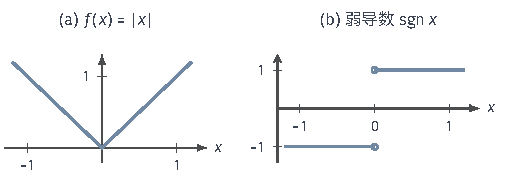
\includegraphics[width=85.7mm]{figures/02-abstract-mathematics/03-function-spaces/tikz/c4-abs-sign/figure.pdf}
  \caption{尖点函数与它的弱导数。(a)~$f(x)=|x|$在原点连续但有尖点；(b)~弱导数$\operatorname{sgn}x$在原点两侧分别为$-1$与$1$，空心点表示原点的取值可以任意约定，弱导数作为等价类不受影响。}
  \label{fig:sob-abs-sign}
\end{figure}

边界项在原点相消，靠的是$|x|$在原点连续。下面的阶跃函数在原点断开，同样的计算会留下一个点读数。

\paragraph{跳跃：阶跃函数}
取$H=\mathbf 1_{(0,\infty)}$。对测试$\varphi$，
\[
 (DT_H)(\varphi)=-\int_{-\infty}^{\infty}H\varphi'\,\mathrm dx=-\int_0^\infty\varphi'\,\mathrm dx=\varphi(0),
\]
所以$DT_H=\delta_0$。$H$在原点外处处可导且经典导数为零，但零函数不是它的弱导数：$\int0\cdot\varphi=0$，而$\delta_0(\varphi)=\varphi(0)$对$\varphi(0)\neq0$的测试不为零。跳跃把变化全部集中在一点上，留下的是测试在跳点的取值。

还要说明$\delta_0$不能由\emph{任何}局部可积函数表示，这样$H$才确实没有弱导数。

\begin{example}[$\delta_0$不是局部可积函数]
\label{ex:sob-delta-not-function}
反设$g\in L^1_{\mathrm{loc}}(\mathbb R)$使$\delta_0=T_g$。取图~\ref{fig:sob-bump-cutoff}(b)中的截断$\chi$，令$\varphi_\varepsilon(x)=\chi(x/\varepsilon)$，$0<\varepsilon\le1$。每个$\varphi_\varepsilon$满足$0\le\varphi_\varepsilon\le1$、$\varphi_\varepsilon(0)=1$，支撑在$[-\varepsilon,\varepsilon]$内（图~\ref{fig:sob-step-delta}(b)）。于是
\[
 1=\delta_0(\varphi_\varepsilon)=\int g\varphi_\varepsilon\,\mathrm dx,\qquad
 \left|\int g\varphi_\varepsilon\,\mathrm dx\right|\le\int_{-\varepsilon}^{\varepsilon}|g|\,\mathrm dx .
\]
$g$在$[-1,1]$上可积，区间$[-\varepsilon,\varepsilon]$的测度趋于零，由积分的绝对连续性，右端趋于零，与左端恒为$1$矛盾。
\end{example}

\begin{figure}[!htb]
  \centering
  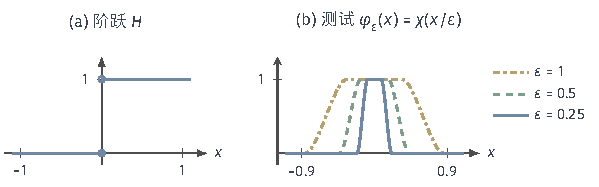
\includegraphics[width=101.5mm]{figures/02-abstract-mathematics/03-function-spaces/tikz/c4-step-delta/figure.pdf}
  \caption{跳跃留下点读数。(a)~阶跃$H=\mathbf 1_{(0,\infty)}$，其广义导数为$\delta_0$。(b)~支撑缩小的测试$\varphi_\varepsilon(x)=\chi(x/\varepsilon)$，$\varepsilon=1,0.5,0.25$：原点值始终为$1$，因此$\delta_0$的读数恒为$1$；而任何局部可积函数与$\varphi_\varepsilon$的配对都被它在越来越短区间上的积分控制，趋于零。}
  \label{fig:sob-step-delta}
\end{figure}

图~\ref{fig:sob-step-delta}把两种读数的差别画了出来：点读数只看原点，测试缩得再窄，读数也不变；函数的积分读数却要乘上支撑的宽度，最终消失。顺带可知$\operatorname{sgn}x=2H-1$的广义导数是$2\delta_0$，所以$|x|$有一阶弱导数，却没有二阶弱导数。

\paragraph{奇异连续变化：Cantor函数}
跳跃的变化集中在一点，函数因而不连续。是否连续函数、且经典导数几乎处处存在，就一定有弱导数？Cantor函数给出否定的回答。

回顾它的构造。从$[0,1]$出发，挖去中间三分之一的开区间$(1/3,2/3)$，在其上令$c=1/2$；对剩下的两个闭区间各自挖去中间三分之一，在$(1/9,2/9)$上令$c=1/4$，在$(7/9,8/9)$上令$c=3/4$；如此继续，第$m$步挖去$2^{m-1}$个长为$3^{-m}$的开区间，并在其上分别取相邻两层平台值的平均。被挖去区间的总长度为$\sum_{m\ge1}2^{m-1}3^{-m}=1$，剩下的Cantor集测度为零。再令$c(0)=0$、$c(1)=1$，并在Cantor集上按单调性补齐，得到$[0,1]$上连续、单调不减的函数$c$（图~\ref{fig:sob-cantor}(a)）。它在每个被挖去的开区间上为常数，所以在测度为$1$的集合上经典导数为零。以概率的语言说，$c$是一个随机变量的分布函数，这个随机变量没有任何单点概率，也没有密度；这一观察可参考\BookChapterRef{chap:random-variables}{卷一“随机变量与概率分布”章}。

\begin{figure}[!htb]
  \centering
  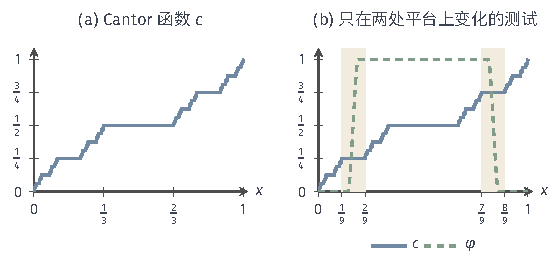
\includegraphics[width=94.7mm]{figures/02-abstract-mathematics/03-function-spaces/tikz/c4-cantor/figure.pdf}
  \caption{Cantor函数没有弱导数。(a)~$c$连续、单调，在被挖去的区间$(\frac13,\frac23)$、$(\frac19,\frac29)$、$(\frac79,\frac89)$等上为常数，在测度为$1$的集合上经典导数为零。(b)~测试$\varphi$（虚线）只在阴影区间$(\frac19,\frac29)$与$(\frac79,\frac89)$内变化，那里$c$分别为$\frac14$与$\frac34$，于是$-\int c\varphi'=-\frac14+\frac34=\frac12$；若$c$有弱导数，这个读数必须为零。}
  \label{fig:sob-cantor}
\end{figure}

\begin{example}[Cantor函数没有弱导数]
\label{ex:sob-cantor}
反设$c$在$(0,1)$上有弱导数$g\in L^1_{\mathrm{loc}}(0,1)$。先在每个被挖去的开区间$I$上看：对支撑在$I$内的测试$\varphi$，$c$在$I$上为常数$c_I$，所以
\[
 \int_Ig\varphi\,\mathrm dx=-\int_Ic_I\,\varphi'\,\mathrm dx=0 .
\]
对开集$I$使用引理~\ref{lem:sob-fundamental}，得$g=0$在$I$上几乎处处成立。被挖去的区间可数个，总长为$1$，因此$g=0$在$(0,1)$上几乎处处成立，从而对所有测试都应有$\int c\varphi'=-\int g\varphi=0$。

再取一个具体测试：$\varphi$在$(1/9,2/9)$内由$0$光滑地升到$1$，在$[2/9,7/9]$上恒为$1$，在$(7/9,8/9)$内光滑地降到$0$（图~\ref{fig:sob-cantor}(b)）。$\varphi'$只在这两个区间内非零，而$c$在那里分别等于$1/4$和$3/4$，所以
\[
 \begin{aligned}
 -\int_0^1c\,\varphi'\,\mathrm dx
 &=-\frac14\int_{1/9}^{2/9}\varphi'\,\mathrm dx-\frac34\int_{7/9}^{8/9}\varphi'\,\mathrm dx\\
 &=-\frac14\cdot1-\frac34\cdot(-1)=\frac12\neq0 ,
 \end{aligned}
\]
矛盾。所以$c$没有弱导数。
\end{example}

读数$1/2$正好是$c$在$[2/9,7/9]$上的增量。实际上，$c$的广义导数是$c$所对应的Lebesgue--Stieltjes测度$\mu_c$（由$\mu_c((s,t])=c(t)-c(s)$确定），它集中在测度为零的Cantor集上，相对Lebesgue测度是奇异的；按第~\ref{sec:measure-lebesgue-decomposition}节的Lebesgue分解（定理~\ref{thm:measure-lebesgue-decomposition}），它没有绝对连续部分，因而不能写成$g\,\mathrm dx$。

\paragraph{三个例子的对照}
表~\ref{tab:sob-three-examples}把三个函数放在一起。三者都几乎处处有经典导数，广义导数也都存在，区别在于广义导数是什么类型的对象。只有$|x|$的广义导数是局部可积函数，才有弱导数；阶跃的变化集中成点质量，Cantor函数的变化集中成奇异连续测度。所以“几乎处处可微”与“弱可微”是两回事：前者只看测度为$1$的集合上的局部斜率，后者要求整体的积分恒等式成立。

\begin{table}[!htb]
 \centering
 \caption{尖点、跳跃与奇异连续变化的对照（区间$(-1,1)$或$(0,1)$上）。}
 \label{tab:sob-three-examples}
 \begin{tabular}{@{}llll@{}}
  \toprule
  函数 & 经典导数 & 广义导数 & 有无弱导数\\
  \midrule
  $|x|$ & 除原点外为$\operatorname{sgn}x$ & $T_{\operatorname{sgn}}$ & 有，$\operatorname{sgn}x$\\
  $H=\mathbf 1_{(0,\infty)}$ & 除原点外为$0$ & $\delta_0$ & 无\\
  Cantor函数$c$ & 几乎处处为$0$ & 奇异测度$\mu_c$ & 无\\
  \bottomrule
 \end{tabular}
\end{table}

$|x|$与另两者的差别在于，它能由自己的导数积分恢复：$|x|=|x_0|+\int_{x_0}^x\operatorname{sgn}t\,\mathrm dt$。阶跃和Cantor函数都做不到这一点，因为它们的经典导数积分出来恒为零。下一小节证明，在一维情形，“能由导数积分恢复”恰好就是弱可微的含义。

\subsection{一维弱导数与绝对连续性}
\label{sec:sob-absolute-continuity}

本小节在有限区间$(a,b)$上工作，记长度$L=b-a$。我们先证明弱导数为零的函数是常数，再借此把弱导数与积分表示联系起来。

\begin{lemma}[弱导数为零的函数]
\label{lem:sob-zero-derivative}
设$f\in L^1_{\mathrm{loc}}(a,b)$，且$\int_a^bf\varphi'\,\mathrm dx=0$对所有$\varphi\in C_c^\infty(a,b)$成立。则存在常数$c$，使$f=c$几乎处处。
\end{lemma}

\begin{proof}
关键是看出哪些测试能写成另一个测试的导数。若$\psi\in C_c^\infty(a,b)$且$\int\psi=0$，则$\varphi(x)=\int_a^x\psi(t)\,\mathrm dt$是光滑的；在$\operatorname{supp}\psi$左侧$\varphi=0$，在其右侧$\varphi=\int\psi=0$，所以$\varphi\in C_c^\infty(a,b)$且$\varphi'=\psi$。于是假设给出：$f$与每个积分为零的测试配对为零。

固定一个积分为$1$的测试$\theta$（例如平移伸缩后的$\rho_\varepsilon$）。任意测试$\psi$可写成$\psi=\bigl(\int\psi\bigr)\theta+\bigl(\psi-(\int\psi)\theta\bigr)$，后一项积分为零，与$f$的配对为零。所以
\[
 \int_a^bf\psi\,\mathrm dx=\Bigl(\int_a^b\psi\,\mathrm dx\Bigr)\int_a^bf\theta\,\mathrm dx=\int_a^bc\,\psi\,\mathrm dx,\qquad c=\int_a^bf\theta\,\mathrm dx .
\]
即$f-c$与所有测试的配对为零，由引理~\ref{lem:sob-fundamental}，$f=c$几乎处处。
\end{proof}

接下来需要一维实分析中的绝对连续函数。称$F:[a,b]\to\mathbb F$\term{绝对连续}（absolutely continuous），若对任意$\varepsilon>0$存在$\delta>0$，使对$[a,b]$中任意有限个两两不交的子区间$(x_i,y_i)$，只要$\sum_i(y_i-x_i)<\delta$，就有$\sum_i|F(y_i)-F(x_i)|<\varepsilon$。它比一致连续强：一致连续只控制一个短区间上的增量，绝对连续控制总长度很短的许多区间上增量之和。Cantor函数连续却不绝对连续：第$m$步剩下$2^m$个闭区间，总长$(2/3)^m$可以任意小，$c$在它们上的增量之和却始终为$1$。

下面使用Lebesgue关于绝对连续函数的微积分基本定理，不在这里证明：若$g\in L^1(a,b)$，则$G(x)=\int_a^xg(t)\,\mathrm dt$在$[a,b]$上绝对连续，且$G'=g$几乎处处；反过来，若$F$在$[a,b]$上绝对连续，则$F$几乎处处可导，$F'\in L^1(a,b)$，并且$F(x)=F(a)+\int_a^xF'(t)\,\mathrm dt$。当$F$单调不减时，这正是说$F$对应的Lebesgue--Stieltjes测度相对Lebesgue测度绝对连续，$F'$是Radon--Nikodym密度（定理~\ref{thm:density-radon-nikodym}）；Cantor函数的测度则完全奇异。

\begin{theorem}[一维弱导数与绝对连续代表]
\label{thm:sob-1d-absolute-continuity}
设$f,g\in L^1(a,b)$。则$g$是$f$的弱导数，当且仅当$f$有一个绝对连续的代表$\tilde f$，满足
\begin{equation}
 \tilde f(y)-\tilde f(x)=\int_x^yg(t)\,\mathrm dt,\qquad a\le x\le y\le b .
 \label{eq:sob-1d-integral-representation}
\end{equation}
此时$\tilde f$在$[a,b]$上唯一，几乎处处有经典导数$\tilde f'=g$。
\end{theorem}

\begin{proof}
先证明累积积分$G(x)=\int_a^xg(t)\,\mathrm dt$以$g$为弱导数。对测试$\varphi$，
\[
 \begin{aligned}
 \int_a^bG\varphi'\,\mathrm dx&=\int_a^b\!\!\int_a^b\mathbf 1_{\{t<x\}}\,g(t)\varphi'(x)\,\mathrm dt\,\mathrm dx\\
 &=\int_a^bg(t)\Bigl(\int_t^b\varphi'(x)\,\mathrm dx\Bigr)\mathrm dt=-\int_a^bg\varphi\,\mathrm dt .
 \end{aligned}
\]
交换积分次序的依据是Fubini定理：被积函数的绝对值不超过$|g(t)|\sup|\varphi'|$，在正方形$[a,b]^2$上可积。最后一步用了$\varphi(b)=0$。

必要性。若$g$是$f$的弱导数，则$f-G$的弱导数为零，由引理~\ref{lem:sob-zero-derivative}，存在常数$c$使$f=c+G$几乎处处。$\tilde f=c+G$绝对连续，并满足式~\eqref{eq:sob-1d-integral-representation}。

充分性。若$f$有满足式~\eqref{eq:sob-1d-integral-representation}的代表，取$x=a$得$\tilde f=\tilde f(a)+G$，常数的弱导数为零，所以$f$的弱导数就是$G$的弱导数$g$。

唯一性：两个连续代表几乎处处相等，在区间的每个非空开子集上不可能处处不同，因而处处相等（非空开区间的Lebesgue测度为正）。$\tilde f'=g$几乎处处来自上面引用的Lebesgue定理。
\end{proof}

定理把一维弱可微性完全翻译成了经典语言：有弱导数，就是能从导数积分回来。把条件放宽到$f,g\in L^1_{\mathrm{loc}}(a,b)$时，同样的论证给出一个在每个紧子区间上绝对连续的代表，只是它可能在端点附近无界，例如$(0,1)$上$f(x)=\ln x$，弱导数$1/x$局部可积但不可积。

\paragraph{积分指数给出Hölder控制}
若进一步知道$g\in L^p(a,b)$，式~\eqref{eq:sob-1d-integral-representation}还能定量地控制$\tilde f$的振荡。对$1<p<\infty$，设$q$为共轭指数，$1/p+1/q=1$。由Hölder不等式，
\begin{equation}
 |\tilde f(y)-\tilde f(x)|\le\int_x^y|g|\cdot1\,\mathrm dt\le\|g\|_{L^p}\,|y-x|^{1/q}=\|g\|_{L^p}\,|y-x|^{1-1/p} .
 \label{eq:sob-1d-holder}
\end{equation}
称满足$|F(x)-F(y)|\le M|x-y|^\gamma$的函数为$\gamma$阶\term{Hölder连续}（Hölder continuous），$0<\gamma\le1$；$\gamma=1$即Lipschitz连续。式~\eqref{eq:sob-1d-holder}说明$\tilde f$是$1-1/p$阶Hölder连续的，指数随$p$增大而增大；$p=\infty$时直接得到Lipschitz控制$|\tilde f(y)-\tilde f(x)|\le\|g\|_{L^\infty}|y-x|$。图~\ref{fig:sob-holder-1d}(a)画出了几种控制函数$h^{1-1/p}$。

\begin{figure}[!htb]
  \centering
  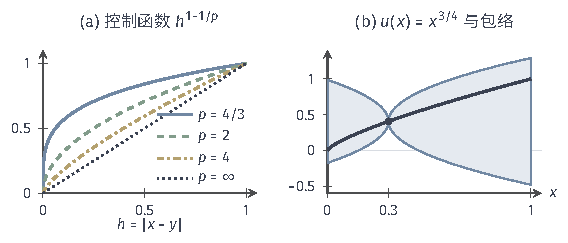
\includegraphics[width=96.2mm]{figures/02-abstract-mathematics/03-function-spaces/tikz/c4-holder-1d/figure.pdf}
  \caption{导数的积分指数控制函数的振荡。(a)~控制函数$h^{1-1/p}$，$p=4/3,2,4,\infty$对应Hölder指数$\frac14,\frac12,\frac34,1$；指数越小，短距离上允许的变化越大。(b)~$u(x)=x^{3/4}$的弱导数$\frac34x^{-1/4}$属于$L^2(0,1)$，$\|u'\|_{L^2}=\sqrt{9/8}\approx1.061$；由式~\eqref{eq:sob-1d-holder}，$u$的图像必须留在以$(0.3,u(0.3))$为顶点的阴影包络$u(0.3)\pm1.061|x-0.3|^{1/2}$内。}
  \label{fig:sob-holder-1d}
\end{figure}

图~\ref{fig:sob-holder-1d}(b)用一个具体函数检验这一估计。$u(x)=x^{3/4}$在原点的经典导数无界，但$u'(x)=\frac34x^{-1/4}$满足$\int_0^1|u'|^2=\frac9{16}\int_0^1x^{-1/2}\,\mathrm dx=\frac98$，所以$u'\in L^2(0,1)$；按定理~\ref{thm:sob-1d-absolute-continuity}它就是弱导数。取$p=2$，式~\eqref{eq:sob-1d-holder}说明$u$的图像整条落在以任一点为顶点、开口为$\sqrt{9/8}\,|x-y|^{1/2}$的包络内，图中以$y=0.3$为例。

$p=1$是例外：此时仍有绝对连续代表，却没有任何正的Hölder指数保证。例如在$(0,1/2)$上取$f(x)=1/\ln(1/x)$，并令$f(0)=0$。它单调增加，$f'(x)=1/\bigl(x\ln^2(1/x)\bigr)$，$\int_0^{1/2}f'=f(1/2)-f(0^+)=1/\ln2$有限，所以$f'\in L^1$。但对任意$\gamma>0$，$h^\gamma\ln(1/h)\to0$（$h\to0^+$），即$f(h)-f(0)=1/\ln(1/h)$比$h^\gamma$大得多，$f$在原点不满足任何正阶Hölder条件。

\paragraph{点值与端点值}
上面的估计还给出用$L^p$大小控制点值的方法。设$f,g\in L^p(a,b)$，$1\le p<\infty$。若$|\tilde f|$处处大于$L^{-1/p}\|f\|_{L^p}$，则$\int|\tilde f|^p>L\cdot L^{-1}\|f\|_{L^p}^p$，矛盾；所以存在$y\in[a,b]$使$|\tilde f(y)|\le L^{-1/p}\|f\|_{L^p}$。对任意$x\in[a,b]$，再由式~\eqref{eq:sob-1d-holder}（$p=1$时直接用$\int|g|$），
\begin{equation}
 \sup_{x\in[a,b]}|\tilde f(x)|\le L^{-1/p}\|f\|_{L^p}+L^{1-1/p}\|g\|_{L^p} .
 \label{eq:sob-1d-sup-bound}
\end{equation}
$p=2$时右端是$L^{-1/2}\|f\|_{L^2}+L^{1/2}\|g\|_{L^2}$。这个估计对闭区间的每一点同时成立，端点也包括在内。

要强调的是，这里的点值都是指唯一的连续代表$\tilde f$的值。在等价类中任取另一个代表，它可以在任意一个零测集上改值，点值便失去意义；正是弱导数的存在，从等价类中选出了唯一一个连续成员。这一结论依赖于一维：在高维，即使函数和全部一阶弱导数都平方可积，函数也可能在一点附近无界，第~\ref{sec:sob-embedding}节将看到维数和积分指数怎样共同决定连续代表是否存在。
